\documentclass[10pt,a4paper,sans]{moderncv} % Changed from 11pt to 10pt

\usepackage{amsfonts,amsthm,amsmath,amssymb,latexsym,xcolor,url}
\usepackage{graphicx,url,pifont,bbding,ifsym,textcomp}
\usepackage{multicol} % For two-column layout in research interests
\usepackage{fontawesome5} % For icons like location
\usepackage[scale=0.935, top=0.5cm, bottom=1.10cm]{geometry} % Adjust margins
\usepackage{fancyhdr} % For custom headers and footers
\usepackage{hyperref} % For clickable links


% Custom page number settings
\pagestyle{fancy}
\fancyhf{} % Clear header and footer
\renewcommand{\headrulewidth}{0pt} % Remove header rule
\renewcommand{\footrulewidth}{0.5pt} % Add footer rule
\fancyfoot[C]{\vspace{0.5cm}\textbf{\thepage}} % Center-align page numbers with spacing

% Disable default moderncv page numbers
\nopagenumbers

\moderncvstyle{classic}
\moderncvcolor{blue}

\renewcommand{\bfseries}{\fontseries{b}\selectfont}
\renewcommand{\itshape}{\fontshape{it}\selectfont}

% Adjust the font sizes of title and address
\renewcommand*{\titlefont}{\fontsize{12pt}{14pt}\selectfont} % Reduced from 14pt to 12pt
\renewcommand*{\addressfont}{\fontsize{8pt}{9pt}\selectfont} % Reduced from 9pt to 8pt

% Custom photo integration
\firstname{\textit{Ali}} % Your first name
\familyname{\textit{NiK}} % Your last name

\renewcommand*{\makecvtitle}{%
  \vspace*{-1.5cm} % Move the entire title block slightly up
  % Photo Section
  \begin{minipage}[t]{0.2\textwidth} % Adjust the width of the photo column
    \vspace*{0.5cm} % Add vertical space to move the photo down
    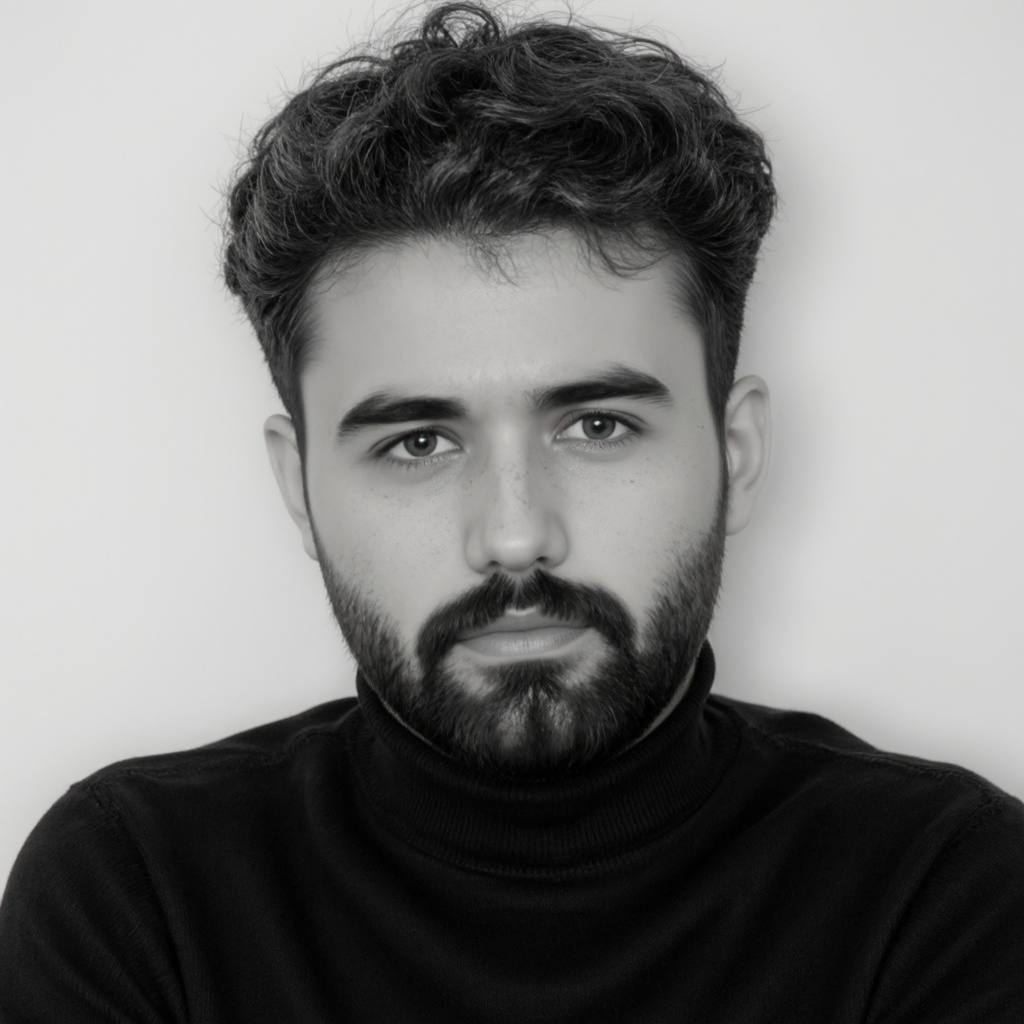
\includegraphics[width=2.9cm]{photo.jpg} % Explicitly set photo width
    \vspace*{-0.1cm}
  \end{minipage}
  \hfill
  % Text Section
  \begin{minipage}[t]{0.75\textwidth} % Adjust the width of the text column
    \vspace*{0.75cm} % Align the text to the top
    {\large\bfseries \firstname~\familyname}\\[-0.3ex] % Reduced from Large to large
    {\Large Ali NiK }\\[-3ex] % Reduced from Large to large
    \addressfont
    \begin{multicols}{2} % Start two-column layout
      \raggedright
      % Column 1
      
\includegraphics[height=1.8em]{house.png}\\ 
      \vspace{-0.43cm}\hspace{0.6cm} 25C App.2.6.1,\\[0.5ex]
      \hspace{0.6cm} Vogeliusweg 25,\\[0.5ex]
      \hspace{0.6cm} 33100 Paderborn,\\[0.5ex]
      \hspace{0.6cm} North Rhine-Westphalia,\\[0.5ex]
      \hspace{0.6cm} Germany
      \\
      \columnbreak
      % Column 2
       
\includegraphics[height=1.4em]{iphone.png} {(+49) 0176 860 44654}\\[1ex]
       
\includegraphics[height=1.3em]{gmail.png} \href{mailto:ali.nazarikhah@iem.fraunhofer.de}{ali.nazarikhah@iem.fraunhofer.de}\\[1ex]
      
\includegraphics[height=1.3em]{linkedin.png} \href{https://linkedin.com/in/ali-nazarikhah}{https://linkedin.com/in/ali-nazarikhah}\\[1ex]
      
\includegraphics[height=1.3em]{github.png} \href{https://github.com/alinik24}{https://github.com/alinazarikhah}
    \end{multicols}
    \vspace*{-0.3cm}
  \end{minipage}
  % Add a horizontal line below the two sections
  \vspace*{-0.2cm}
  \line(1,0){557}

}

\begin{document}
\makecvtitle 




\section{\faGraduationCap{} EDUCATION}

%Entry 1
\cvitem{
\raggedright
\makebox[5cm][l]{\footnotesize \faIcon{calendar-day} \colorbox{yellow!30}{2023/24 -- Present}\hspace*{0.13cm}\textbf{MSc}} \\
\makebox[5cm][l]{\footnotesize\faMapMarker*{} 
\includegraphics[height=0.8em]{it.png} Italy / 
\includegraphics[height=0.8em]{de.png} Germany}
}{
$\bullet$ \textbf{Engineering in Computer Science [EiCS]} \newline 
{

\includegraphics[height=1.5em]{sap.png}\hspace{0.05em} 
\includegraphics[height=1.4em]{UPb.png} Department of Information Engineering, Computer Science, and Statistics, Sapienza University of Rome / Paderborn University} \newline
{\scriptsize \faInfoCircle{}} \footnotesize Pursued concurrently with MSc in Energy Engineering \newline% Changed small to footnotesize
{$\bullet$ \footnotesize Thesis title:} \footnotesize TBD
 \newline % Changed small to footnotesize
{$\bullet$ \footnotesize Supervisor:} \footnotesize TBD \newline % Changed small to footnotesize
{$\bullet$ \footnotesize GPA:} \footnotesize 90/110 [3.6/4.0 - all coursework completed; thesis pending]
}
\vspace{0.35cm} 


% Entry 2
\cvitem{
\raggedright
\makebox[5cm][l]{\footnotesize\faIcon{calendar-day} 2022/23 -- 2025/26\hspace*{0.23cm}\textbf{MSc}} \\ % Changed small to footnotesize
\makebox[5cm][l]{\footnotesize\faMapMarker*{} 
\includegraphics[height=0.8em]{it.png} Italy}
}{
$\bullet$ \textbf{Energy Engineering [EE]} \newline
{
\includegraphics[height=1.5em]{sap.png} Department of Astronautical, Electrical and Energy Engineering, Sapienza University of Rome} \newline
{$\bullet$ \footnotesize Thesis title:} \footnotesize Energy Demand Modeling of Industrial Furnaces for Energy Efficiency Assessment;
Specification and Validation in roller hearth furnace
 \newline % Changed small to footnotesize
{$\bullet$ \footnotesize Supervisor:} \footnotesize Prof. Luigi Martirano \newline % Changed small to footnotesize
{$\bullet$ \footnotesize GPA:} \footnotesize 110/110 [4.0/4.0]
}
\vspace{0.35cm}

% Entry 3
\cvitem{
\raggedright
\makebox[5cm][l]{\footnotesize\faIcon{calendar-day} 2015/16 -- 2020/21\hspace*{0.23cm}\textbf{BSc}} \\ % Changed small to footnotesize
\makebox[5cm][l]{\footnotesize\faMapMarker*{} 
\includegraphics[height=0.8em]{ir.png} Iran}
}{
$\bullet$ \textbf{Chemical Engineering [CE]} \newline 
{

\includegraphics[height=1.5em]{Sahand University of Technology.png} Department of Chemical Engineering, Sahand University of Technology (SUT)} \newline
{$\bullet$ \footnotesize Thesis Title:} \footnotesize Investigated the effects of electrochemical processes and synthesized zeolite nano-adsorbents on membrane fouling in a membrane bioreactor \newline % Changed small to footnotesize
{$\bullet$ \footnotesize Supervisor:} \footnotesize Prof. Hossein Hazrati \newline % Changed small to footnotesize
{$\bullet$ \footnotesize GPA:} \footnotesize 18.06/20 [3.85/4.0] [4.0/4.0]
}

\section{\faGlobe{} RESEARCH INTERESTS}

\begin{multicols}{2}
\cvitem{}{\faBolt{} Energy Conversion and System Optimization}
\cvitem{}{\faSolarPanel{} Renewable Energy Systems and Sustainability}
\cvitem{}{\faBuilding{} Smart Grids and Power Systems in Smart Buildings}
\cvitem{}{\faCode{} Software Development For Energy Monitoring, \newline Optimization, and Predictive Maintenance}
\columnbreak
\cvitem{}{\faBrain{} AI and ML Applications}
\cvitem{}{\faDatabase{} Data-Driven Decision-Making}
\cvitem{}{\faMicrochip{} Internet of Things (IoT)}
\cvitem{}{\faCubes{} Blockchain Applications}
\cvitem{}{\faEdit{} UI/UX and Product Design}
\end{multicols}

\section{\faCogs{} EXPERIENCE}

% GenAI Incubator entry
\cvitem{
\raggedright
\makebox[5cm][l]{\footnotesize \faIcon{calendar-day} \colorbox{yellow!30}{Mar 2025 -- Present}} \\ % Changed small to footnotesize
\makebox[5cm][l]{\faMapMarker*{} \footnotesize Paderborn, Germany} % Changed small to footnotesize
}{$\bullet$ \textbf{Research Assistant} 
\newline{

\includegraphics[height=1.5em]{fraunhofer.png}\ GenAI Incubator, Fraunhofer IEM} \newline \footnotesize Conducting research on Generative AI \& ML-driven solutions for industrial challenges, leveraging data-driven approaches and decision-making to enhance automation and operational efficiency.
} % Changed small to footnotesize

% Research Intern entry
\cvitem{
\raggedright
\makebox[5cm][l]{\footnotesize \faIcon{calendar-day} Feb 2024 -- Jun 2024} \\ % Changed small to footnotesize
\makebox[5cm][l]{\faMapMarker*{} \footnotesize Rome, Italy} % Changed small to footnotesize
}{$\bullet$ \textbf{Research Assistant}
\newline{

\includegraphics[height=0.9em]{enea.png}\ Energy and Environmental Technology, Italian National Agency for New Technologies (ENEA)} \newline \footnotesize Conducted energy efficiency assessments, analyzed RE integration, developed sustainable energy solutions, and contributed to research on emission reduction technologies aligned with EU environmental goals.} % Changed small to footnotesize

% Energy Efficiency Consultant entry
\cvitem{
\raggedright
\makebox[5cm][l]{\footnotesize \faIcon{calendar-day} Jul 2021 -- Oct 2021} \\ % Changed small to footnotesize
\makebox[5cm][l]{\faMapMarker*{} \footnotesize Tabriz, Iran} % Changed small to footnotesize
}{$\bullet$ \textbf{Energy Efficiency Consultant} 
\newline{\scalebox{1.6}{\faIndustry}\ Talaaye Daaraane Moderne Shomal Gharb} \newline \footnotesize Conducted industrial energy audits, analyzed energy consumption patterns, proposed efficiency strategies, and prepared actionable plans to support sustainable development.} % Changed small to footnotesize

% Project Manager entry
\cvitem{
\raggedright
\makebox[5cm][l]{\footnotesize \faIcon{calendar-day} May 2021 -- Jun 2021} \\ % Changed small to footnotesize
\makebox[5cm][l]{\faMapMarker*{} \footnotesize Kharg Island, Iran} % Changed small to footnotesize
}{$\bullet$ \textbf{Project Control Engineer} 
\newline{

\includegraphics[height=1.5em]{kharg.png}\ Kharg Petrochemical Company Limited} \newline \footnotesize Supported project management during major overhaul operations by tracking schedules, supporting resource planning, ensuring HSE and regulatory compliance, and coordinating multidisciplinary teams to to meet project milestones.} % Changed small to footnotesize

% Process Engineering Technician entry
\cvitem{
\raggedright
\makebox[5cm][l]{\footnotesize \faIcon{calendar-day} Jan 2021 -- Apr 2021} \\ % Changed small to footnotesize
\makebox[5cm][l]{\faMapMarker*{} \footnotesize Mahshahr Port, Iran} % Changed small to footnotesize
}{$\bullet$ \textbf{Process Engineer} 
\newline{

\includegraphics[height=1.1em]{bandarimam.png}\ Bandar Imam Petrochemical Complex} \newline \footnotesize Enhanced plant operational performance by designing preventive maintenance strategies and minimizing downtime through structured troubleshooting and process analysis.} % Changed small to footnotesize

% Environmental Researcher entry
\cvitem{
\raggedright
\makebox[5cm][l]{\footnotesize \faIcon{calendar-day} Jan 2017 -- Mar 2020} \\ % Changed small to footnotesize
\makebox[5cm][l]{\faMapMarker*{} \footnotesize Tabriz, Iran} % Changed small to footnotesize
}{$\bullet$ \textbf{Research Assistant – Sustainable Process Engineering} 
\newline{

\includegraphics[height=1.5em]{Sahand University of Technology.png}\ Environmental Engineering Research Center (EERC), SUT} \newline \footnotesize Conducted research on sustainable industrial waste management and developed catalyst regeneration and synthesis strategies to replicate the performance of imported refinery catalysts under supply constraints.} % Changed small to footnotesize

% Process Engineering Intern entry
\cvitem{
\raggedright
\makebox[5cm][l]{\footnotesize \faIcon{calendar-day} Jun 2017 -- Aug 2017} \\ % Changed small to footnotesize
\makebox[5cm][l]{\faMapMarker*{} \footnotesize Mohr, Iran} % Changed small to footnotesize
}{$\bullet$ \textbf{Process Engineering Intern} 
\newline{

\includegraphics[height=1.7em]{National_Iranian.png}\ Parsian Gas Refinery Company} \newline \footnotesize Developed expertise in PFDs and P\&IDs, evaluated refinery processes, and proposed energy efficiency improvements, including flare gas recovery research and process simulations.} % Changed small to footnotesize

\section{\faProjectDiagram{} PROJECTS}

\cvitem{\faLaptopCode{} EiCS}{%
    $\bullet$ \textbf\footnotesize{Digital Project Management Transformation at Benteler — Legacy Excel digitalization, structured data modeling, centralized project knowledge base creation, and RAG-based information retrieval system design.}
}

\cvitem{}{%
    $\bullet$ \textbf\footnotesize{Predictive Quality Modeling for SMT Production (FORVIA HELLA) — Development of a machine learning pipeline for early defect detection in PCB manufacturing using supervised learning and Explainable AI to classify product quality and enable interpretable decision support.}
}

\cvitem{}{%
    $\bullet$ \textbf\footnotesize{Electrical Schema Digitalization for Industrial Automation (HIK) — Conversion of electrical schematics into structured, machine-readable schemas for automation, interoperability, and downstream engineering integration.}
}

\cvitem{}{%
    $\bullet$ \textbf\footnotesize{Machine Parameter Identification and Data Mapping in Battery Cell Production — Structuring, optimization, and consistency analysis of machine parameters to support scalable digital production workflows.}
}

\cvitem{}{%
    $\bullet$ \textbf\footnotesize{Legal-Tech SaaS Platform Development (Concept \& Prototype) — Solution architecture design, service workflow definition, and scalability analysis for administrative and legal process automation in Germany.}
}

\cvitem{}{%
    $\bullet$ \textbf\footnotesize{Physiognomy-Based Personality Analysis Application — Machine learning concept development, UI/UX optimization, and interactive prototyping using Figma.}
}

\cvitem{}{%
    $\bullet$ \textbf\footnotesize{Senior+ — AI-Driven HR Platform — Design of adaptive onboarding and knowledge retention workflows using personalized, data-driven digital processes.}
}

\cvitem{}{%
    $\bullet$ \textbf\footnotesize{Administrative Digitalization Platform for the Public Sector — Digital onboarding system design, process automation, usability optimization, and cross-departmental workflow coordination.}
}

\cvitem{}{%
    $\bullet$ \textbf\footnotesize{Personalized Deep-Research Platform for Idea Scouting — Development of a data-driven research system for personalized information retrieval, structured market analysis, and early-stage idea evaluation.}
}


\vspace{0.25cm}

\cvitem{\faBolt{} EE}{%
    $\bullet$ \textbf\footnotesize{Techno-Economic Assessment of a Solar-Powered Hybrid RO-MED Desalination System in Bushehr, Iran.}
}

\cvitem{}{%
    $\bullet$ \textbf\footnotesize{Aerodynamic Optimization of Wind Turbine Blades Using Computational Fluid Dynamics (Python/OpenFOAM).}
}

\cvitem{}{%
    $\bullet$ \textbf\footnotesize{Sustainable Energy Transition via Geothermal Power — Resource assessment, plant design, and feasibility study for Lumut Balai, Indonesia (DoubleCalc 2D).}
}

\cvitem{}{%
    $\bullet$ \textbf\footnotesize{Tidal Energy Harvester Design — Hydrodynamic analysis and performance prediction (OceanusLink).}
}

\cvitem{}{%
    $\bullet$ \textbf\footnotesize{Hybrid Renewable Microgrid Design for Rural Namibia — Resilience analysis under extreme weather conditions (HOMER Pro/UQ).}
}

\cvitem{}{%
    $\bullet$ \textbf\footnotesize{Energy Audit and Optimization at Campus X, Rome — Data-driven real-time performance analysis and multi-dimensional impact assessment.}
}

\cvitem{}{%
    $\bullet$ \textbf\footnotesize{DüsselPulse — AI-driven smart city solutions across energy, economy, mobility, environment, and community using data-driven decision-making and uncertainty quantification.}
}

\vspace{0.25cm}

\cvitem{\faIndustry{} CE}{%
    $\bullet$ \textbf\footnotesize{Techno-Economic Analysis and Heat Recovery Optimization of Solid Oxide Electrolyzers for Green Hydrogen (PRO/II).}
}

\cvitem{}{%
    $\bullet$ \textbf\footnotesize{Flare Gas Recovery System Optimization in Refineries (Aspen HYSYS).}
}

\cvitem{}{%
    $\bullet$ \textbf\footnotesize{Business Plan for Molecular Sieve-Based Catalyst Recovery in the Adsorption Unit of the Persian Gas Refinery — Plant design and economic assessment.}
}

\cvitem{}{%
    $\bullet$ \textbf\footnotesize{Process Simulation and Optimization of the Reformer Unit in Kharg Petrochemical Complex (Aspen HYSYS).}
}

\cvitem{}{%
    $\bullet$ \textbf\footnotesize{CFD Simulation of Stirred Tanks — Comparison of turbulence models and impeller designs using COMSOL.}
}

\cvitem{}{%
    $\bullet$ \textbf\footnotesize{Two-Phase Flow Simulation and Enhanced Recovery Strategies for Arash Gas Field, Iran (ECLIPSE 300).}
}


\section{\faRocket{} SKILLS}
\cvitem{\hspace*{-1cm}\textbf{\faBolt{} EE \& \faIndustry{} CE} \cvskill{4}}
{     
    \footnotesize Python (pvlib, Cantera, sympy), MATLAB, OpenFOAM, COMSOL Multiphysics, Aspen HYSYS, Pro/II , LabVIEW, PSS/E, HOMER Energy, Carrier HAP, Revit (BIM),    
    %EnergyPlus,    
    RETScreen Expert, PVsyst, AI-driven industrial analytics (Seeq), digital twins (ANSYS Twin Builder), MS Project, %Jira,   
    Microsoft Office Suite %, Primavera P6
    }
    
\cvitem{\hspace*{0}\textbf{\faLaptopCode{} EiCS} \cvskill{2}}
{$\bullet$ \textbf{AI/ML Engineering} \hfill\cvskill{3} \newline \footnotesize LLMs, NLP, Generative AI (RAG, Diffusion Models), %Multimodal AI, 
PyTorch, TensorFlow, Hugging Face, LangChain, %Cloud AI Platforms (Vertex AI),
MLOps (MLflow, W\&B),  Fine-tuning \& Quantization, LM Studio, ComfyUI, n8n\newline % Changed small to footnotesize
$\bullet$ \textbf{Data Science} \hfill\cvskill{2} \newline
\footnotesize Python (Polars, PySpark), R, SQL (incl. BigQuery), %Snowflake, Apache Spark, 
AutoML frameworks, DBT, Image processing and data annotation workflows (Label Studio) %Streamlit/Plotly Dash, Airflow,
Jupyter \newline % Changed small to footnotesize
$\bullet$ \textbf{Cloud \& Development} \hfill\cvskill{3} \newline \footnotesize AWS, Azure, Docker/K8s, %React/Next.js,
FastAPI, AI-enhanced DevOps, Devin AI, Vercel, Expo, Figma, HTML5, CSS3} % Changed small to footnotesize

\section{}
\vspace{-1cm}
\begin{center}
    \begin{minipage}[t]{0.5\textwidth} % Left Column (Workshops)
        \subsection{\faChalkboardTeacher{} WORKSHOPS \& CERTIFICATES} 
        \vspace{-0.1cm}
        \cvitem{
        \raggedright
        \makebox[5cm][l]{
\includegraphics[height=1em]{udd.png}Udemy}}{\footnotesize $\bullet$ AI Agents and Advanced Workflow Automation}
        \cvitem{}{\footnotesize $\bullet$ GenAI for Business Analysis: LLM Fine-Tuning and RAG Architectures}  
        \cvitem{
        \raggedright
        \makebox[5cm][l]{ 
\includegraphics[height=0.95em]{c.png} Coursera}}{\footnotesize $\bullet$ Deep Learning (Neural Networks, CNNs, Sequence Models)} 
        \cvitem{}{\footnotesize $\bullet$ Natural Language Processing}
        \cvitem{}{\footnotesize $\bullet$ Sentiment Analysis with Deep Learning} 
        \cvitem{}{\footnotesize $\bullet$ Game Design and Development}
        \cvitem{}{\footnotesize $\bullet$ Ethical Hacking Essentials (EHE)} 
        \cvitem{}{\footnotesize $\bullet$ Web3 and Blockchain} 
        \cvitem{}{\footnotesize $\bullet$ Programming the Internet of Things (IoT)} 
        \cvitem{
        \raggedright
        \makebox[5cm][l]{ \faMapMarker*{} \footnotesize Kharg Island, Iran}}{\footnotesize $\bullet$ PFD and P\&ID Sheets in Process Engineering, Kharg Petrochemical Complex} 
        \cvitem{}{\footnotesize $\bullet$ HSE Principles and Practices, Kharg Petrochemical Complex} 
    \end{minipage}%
    \hfill
    \begin{minipage}[t]{0.5\textwidth} % Right Column (Languages)
\subsection{\faComments{} LANGUAGES}

\cvitem{}{\begin{tabular}{@{}p{2.8cm}@{\hskip 10pt}l}
    $\bullet$ English     & \cvskill{5} \footnotesize C2 \\[0.5em]
    $\bullet$ German      & \cvskill{3} \footnotesize B1 \\[0.5em]
    $\bullet$ Italian     & \cvskill{2} \footnotesize A2 \\[0.5em]
    $\bullet$ Arabic      & \cvskill{2} \footnotesize A2 \\[0.5em]
    $\bullet$ Persian     & \cvskill{5} \footnotesize C2 \\[0.5em]
    $\bullet$ Turkish     & \cvskill{2} \footnotesize A2
\end{tabular}}
\end{minipage}
\end{center}

\section{\faMedal{} HONORS \& AWARDS}

\cvitem{}{\footnotesize $\bullet$ Finalist, XChange4Industry Makeathon (Fraunhofer IEM) \newline
{\scriptsize (48-hour industry challenge resulting in a working prototype for secure, sovereign, and interoperable manufacturing data exchange aligned with Gaia-X and Factory-X principles.)}}

\cvitem{}{\footnotesize $\bullet$ Graduated with highest distinction, MSc Energy Engineering, Sapienza University of Rome \newline
{\scriptsize (First foreign student to concurrently pursue two engineering Master’s degrees, achieving full distinction (110/110) within the standard duration and ranking first among the cohort in the MSc Energy Engineering program.)}}



\cvitem{}{\footnotesize $\bullet$ Finalist at Demo Day, DOCK3 Startup Incubator, Rome, Italy \newline
{\scriptsize (Immersed in a fast-paced startup ecosystem, strengthening hands-on experience in AI, ML, edge computing, and emerging digital technologies, while fostering adaptability and a strong problem-solving mindset.)}}

\cvitem{}{\footnotesize $\bullet$ Ranking 2nd among my cohort in the BSc Chemical Engineering program, Sahand University of Technology}

\cvitem{}{\footnotesize $\bullet$ Awarded the prestigious ``Financial Educational Award'' by Iran’s National Elites Foundation}

\cvitem{}{\footnotesize $\bullet$ Ranked in the top 1\% of 185,000 participants in the Iranian National University Entrance Exam and awarded a full tuition waiver for Bachelor’s studies}

\section{\faGamepad{} HOBBIES}

\begin{multicols}{3}
\cvitem{}{
\begin{tabular}{@{}l@{\hskip 10pt}l}
    \faYoutube{} \scriptsize Online Learning (YouTube, MOOCs) \\
    \faPodcast{} \scriptsize Tech Innovations \& Startup Culture \\ [-0.3em]
    \scriptsize newline (News, Podcasts, Articles)
    \end{tabular}}
\columnbreak
\cvitem{}{
\begin{tabular}{@{}l@{\hskip 10pt}l}
    \faBook{} \scriptsize Reading \\
    \faChartLine{} \scriptsize Financial Market Analysis \\
\end{tabular}}
\columnbreak
\cvitem{}{
\begin{tabular}{@{}l@{\hskip 10pt}l}
     \faGuitar{} \scriptsize Classical Guitar \\
     \faDumbbell{} \scriptsize Fitness \& Sports
\end{tabular}}
\end{multicols}

\section{\faUser{} REFEREES 
\hfill {\normalsize \faFilePdf{}} \href{https://drive.google.com/file/d/1bWt9w5Vz_ohXiWX7r_eprzJ98oJn6Mc2/view?usp=sharing}{\large{Recommendation Letters}}
}


\vspace{0.65em}

% --- alignment control for email lines ---
\newcommand{\EmailAlign}{\hspace*{9 cm}}

\cvitem{Professional}{
\faBriefcase{} \textbf{Tommy Falkowski} \newline
Head of GenAI Incubator, Fraunhofer-Institut für Entwurfstechnik Mechatronik IEM, Paderborn, Germany \newline
\EmailAlign \faEnvelope{} \texttt{tommy.falkowski@iem.fraunhofer.de}
}
\vspace{0.25cm}

\cvitem{Academic--MSc}{
\faGraduationCap{} \textbf{Prof.\ Leonardo Micheli} \newline
Associate Professor, Department of Astronautical, Electrical, and Energy Engineering (DIAEE), Sapienza University of Rome, Rome, Italy \newline
\EmailAlign \faEnvelope{} \texttt{leonardo.micheli@uniroma1.it}
}
\vspace{0.25cm}

\cvitem{Academic--BSc}{
\faGraduationCap{} \textbf{Prof.\ Mohammad Zabihi} \newline
Associate Professor, Department of Chemical Engineering, Sahand University of Technology (SUT), Tabriz, Iran \newline
\EmailAlign \faEnvelope{} \texttt{zabihi@sut.ac.ir}
}
\vspace{0.25cm}

\cvitem{Professional}{
\faBriefcase{} \textbf{Eng.\ Mohammad Torabi} \newline
Overhaul Planning and Project Control Director, Khark Petrochemical Complex, Khark Island, Iran \newline
\EmailAlign \faEnvelope{} \texttt{mohammad.torabi@khipc.com}
}

\end{document}

